\section{Symetrické šifry}
\hyphenation{AES-NI}
Šifra s tajným klíčem je taková šifra, u nichž pro dešifrování nějaké informace je povětšinou identický jako klíč pro zašifrování. Bezpečnost a integrita dat utě chto šifer je dána tím,že příslušný klíč je znám pouze oprávněným stranám \parencite{tesar2021}.

Jedním z nejznámějších systémů založených na symetrické kryptografii jsou šifry zpracovávající data po blocích. Standard AES (Advanced Encryption Standard) není bloková šifra, jak je často ve veřejných publikacích zmiňováno. Jedná se totiž o standard, vydaný americkým institutem NIST (National Institute of Standards and Technology), který používá symetrickou blokovou šifru pod názvem Rijndael. Algoritmus provádí několik předem definovaných cyklů (rund), které zahrnují substituce, a permutace s jedním klíčem. Princip funkce těchto jednotlivých etap je složitý na popis a je v podstatě důležitý jen pro ty, kteří tento algoritmus implementují do svého systému \parencite {nist2023}.

V praxi se AES nejčastěji využívá k šifrování disků nebo zabezpečení síťové komunikace. Pro urychlení výpočtu tohoto algoritmu byly od roku 2010 zavedeny speciální instrukce do procesorů, například Intel \textregistered{} AES-NI, které jsou dostupné nejen na procesorech od Intelu, ale také u procesorů AMD a dalších výrobců čipů. Tyto instrukce jsou implementovány i v mobilních zařízeních, což umožňuje efektivnější šifrování a dešifrování dat, potřebnou pro nižší spotřebu energie \textcite{abdallah2020}.

Hlavním problémem těchto systémů však stále zůstává: Jak můžeme bezpečně sdílet příslušný klíč, aniž by hrozilo jeho prozrazení třetí straně, a ověřit, že druhá strana je opravdu ta, za kterou se vydává?

\subsection{Problém distribuce klíčů}
\label{sec:distribuce-klicu}
\hyphenation{Diffie-Hellman}
Distribuce klíčů je základním problémem při používání symetrických šifer, protože pro šifrování a dešifrování se většinou používá stejný \enquote{tajný} klíč. Bezpečnost komunikace mezi odesílatelem a příjemcem závisí na uchování tajnosti tohoto klíče, jelikož pokud by neoprávněná strana získala onen klíč, mohla by snadno tuto komunikaci odposlouchávat \parencite{tesar2021}.

Představme si situaci, kdy klient (např. webový prohlížeč), se pokouší získat přístup k serveru a je třeba zabezpečit tento komunikační kanál. Data, která jsou mezi stranami sdílena, jsou většinou většího objemu a komunikace probíhá neustále, takže není efektivní používat asymetrickou kryptografii. K tomu, aby mohl klient a server bezpečně komunikovat, je třeba vyměnit tajný klíč tzv. secret key \textcite{wikijs2024}. Vzniká zde otázka: \enquote{Jak bezpečně vyměnit tajný klíč přes nezabezpečený kanál, jako je transportní vrstva sítě?} Jedním z efektivních řešení je právě Diffie-Hellmanův protokol, jenž je využíván napříč mnoha kryptografickými protokoly.

\subsection{Diffie-Hellmanův protokol}
\label{sec:diffie-hellman}

Jak uvádí \textcite{diffie1976}, princip tohoto protokolu spočívá ve vytvoření bezpečného klíče mezi dvěma stranami bez nutnosti předchozího sdílení tajných klíčů. Tento proces umožňuje stranám (např. klientovi a serveru) bezpečně si vyměnit šifrovací klíče přes veřejný kanál a zajistit tak důvěrnost při komunikaci.

Princip funkce výměny klíčů mezi dvěma stranami, v našem případě klient-server, je dle \textcite{diffie1976}, popsán následujícím způsobem: 

\begin{enumerate}
  \item \textbf{Volba veřejných parametrů:} Obě strany si zvolí dvě veřejné hodnoty, které jsou známé všem účastníkům komunikace. Tyto hodnoty jsou označeny jako \(g\) (základna) a \(p\) (prvočíslo, často označované jako modul). Parametry musí být vybrány tak, aby zaručovaly bezpečnost celého protokolu. V praxi se obvykle volí prvočíslo \(p\) s délkou alespoň 2048 bitů (či 4096-bitová čísla) a malá hodnota pro \(g\).
  
  \item \textbf{Výběr tajných čísel:} Každá strana si následně náhodně vybere své vlastní tajné číslo, přičemž klient zvolí číslo \(a\) a server číslo \(b\). Tato čísla jsou vybírána z rozsahu \(1 \leq a, b \leq p-2\) a musí být dostatečně velká a náhodná, aby byla zajištěna bezpečnost výměny. Tyto hodnoty nikdy nejsou sdíleny s druhou stranou.
  
  \item \textbf{Výpočet veřejných hodnot:} Na základě svých tajných čísel a veřejných parametrů obě strany spočítají své veřejné hodnoty následujicím způsobem. Klient vypočítá \(A = g^a \mod p\) a server \(B = g^b \mod p\). Výsledné hodnoty \(A\) a \(B\) jsou vyměněny mezi stranami.
  
  \item \textbf{Vytvoření sdíleného klíče:} Po výměně veřejných hodnot každá strana využije své tajné číslo a přijatou veřejnou hodnotu k výpočtu sdíleného klíče. Klient spočítá \(s = B^a \mod p\) a server \(s = A^b \mod p\). Díky vlastnostem modulární aritmetiky jsou obě hodnoty shodné, čímž obě strany získají stejný sdílený tajný klíč.
\end{enumerate}

I když jsou veřejné hodnoty \(A\) a \(B\) přenášeny přes nechráněný kanál, zpětné určení tajných čísel \(a\) a \(b\) je extrémně náročné. Tento problém, známý jako problém diskrétního logaritmu v grupě zbytkových tříd modulo \(p\), má pro klasické počítače exponenciální složitost, což znamená, že výpočet je s rostoucí velikostí čísel extrémně časově náročný. Pro moderní aplikace se pak volí dostatečně velká prvočísla, aby byl tento problém prakticky neřešitelný. Potenciální hrozbou mohou být pouze kvantové počítače, které by mohly pomocí specifických algoritmů, jako je Shorův algoritmus (popsaný více v kapitole \hyperref[sec:postkvantova-kryptografie]{Postkvantová kryptografie}), snížit výpočetní složitost tohoto problému na polynomiální úroveň.

\begin{figure}[htbp]
    \centering
    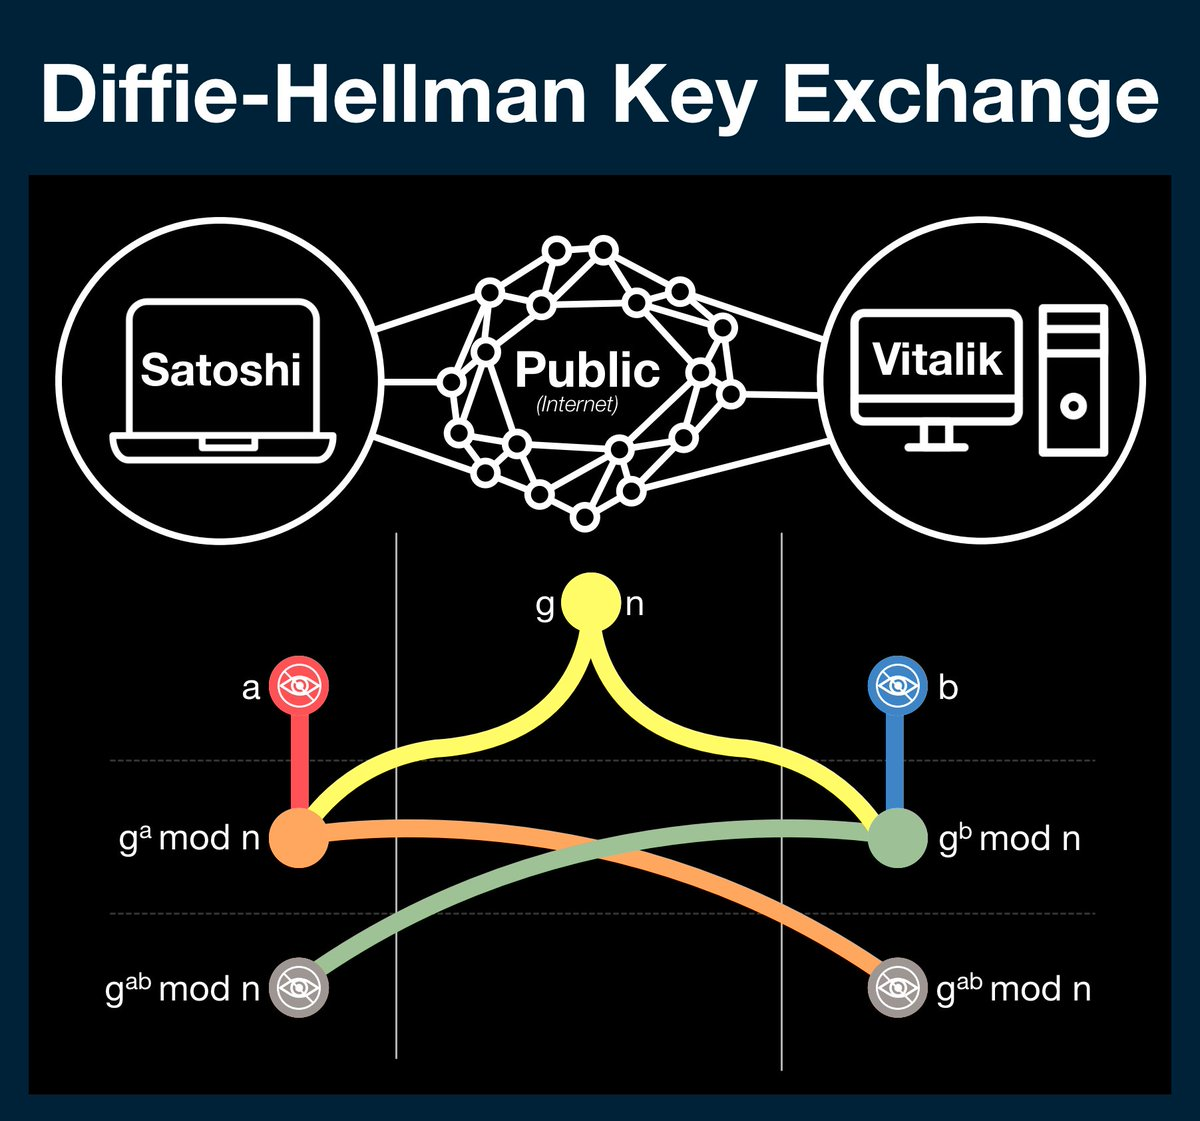
\includegraphics[width=1\textwidth]{\FIGURES/diffie-hellman-1.jpeg}
    \caption{Schéma Diffie-Hellmanova protokolu. Zdroj: \parencite{diffie-hellman-1}}
    \label{fig:diffie-hellman}
  \end{figure}

\newpage